\documentclass{llncs}
\usepackage{pslatex}	
\usepackage{tikz}	
\usetikzlibrary{calc}
\usetikzlibrary{shapes.geometric}
\usetikzlibrary{shapes.arrows}
\usetikzlibrary{shapes.misc}
\usetikzlibrary{fit}

\begin{document}

\begin{center}
\begin{tikzpicture}[font=\small,overlay,
mycirclex/.style={draw, circle, minimum size=0.70em, inner sep = 0mm}, 
mydiamond/.style={draw, diamond, minimum size=0.78em, inner sep = 0mm}, 
myrectang/.style={draw, rectangle, minimum size=0.60em, inner sep = 0mm}, 
>=stealth]

\def\cola{blue}
\def\colb{brown}
\def\colc{green}
\def\cold{violet}
\def\colx{black}

\def\len{0.65cm}

% G1
\begin{scope}[xshift=-4.8cm]
\begin{scope}[local bounding box=bbox]
\node at (-0.5 * \len, 0) {$G_1$};
\draw[blue,  ->, line width=0.1cm] (0 * \len, 0) to node[above]{$a$}  (1 * \len, 0);
\draw[brown, ->, line width=0.1cm] (1 * \len, 0) to node[above]{$b$}  (2 * \len, 0);
\draw[green, ->, line width=0.1cm] (2 * \len, 0) to node[above]{$c$}  (3 * \len, 0);
\draw[violet,  ->, line width=0.1cm] (3 * \len, 0) to node[above]{$d$}  (4 * \len, 0);
\end{scope}
%\draw[rounded corners] ($(bbox.south west) - (0.00cm, 0.25cm)$) rectangle ($(bbox.north east) + (0.1cm, 0)$);
%\node at ($(bbox.south) - (0.00cm, 0.2cm)$) [label=below:{$G_2 - G_1 = \{c\}$}]{};

% G2
\begin{scope}[local bounding box=cbox, yshift=-2.82cm, xshift=0cm]
\node at (-0.5 * \len, 0) {$G_2$};
\draw[brown,  ->, line width=0.1cm] (0 * \len, 0) to node[above]{$b$}  (1 * \len, 0);
\draw[blue, <-, line width=0.1cm] (1 * \len, 0) to node[above]{$-a$}  (2 * \len, 0);
\draw[green, ->, line width=0.1cm] (2 * \len, 0) to node[above]{$c$}  (3 * \len, 0);
\draw[violet,  <-, line width=0.1cm] (3 * \len, 0) to node[above]{$-d$}  (4 * \len, 0);
\end{scope}
%\draw[rounded corners] ($(cbox.south west) - (0.00cm, 0.25cm)$) rectangle ($(cbox.north east) + (0.1cm, 0.0cm)$);
%\node at ($(cbox.north) + (0.00cm, 0.0cm)$) [label=above:{$G_1 - G_2 = \{a\}$}]{};


% adjacency graph
\begin{scope}[local bounding box=cbox, xscale=1.4, yscale=1.2, xshift=2.8cm,yshift=-0.11cm]
\node[myrectang, color=\colx, fill=\colx, draw] (e1) at (0.0cm, 0.0cm) {};
\node[mydiamond, color=\cola, fill=\cola, draw] (e2) at (0.3cm, 0.0cm) {};
\node at (e1.east) [label=above:{$\{0,a_t\}$}]{};

\node[mycirclex, color=\cola, fill=\cola, draw] (e3) at (1.0cm, 0.0cm) {};
\node[mydiamond, color=\colb, fill=\colb, draw] (e4) at (1.3cm, 0.0cm) {};
\node at (e3.east) [label=above:{$\{a_h,b_t\}$}]{};

\node[mycirclex, color=\colb, fill=\colb, draw] (e5) at (2.0cm, 0.0cm) {};
\node[mydiamond, color=\colc, fill=\colc, draw] (e6) at (2.3cm, 0.0cm) {};
\node at (e5.east) [label=above:{$\{b_h,c_t\}$}]{};

\node[mycirclex, color=\colc, fill=\colc, draw] (e7) at (3.0cm, 0.0cm) {};
\node[mydiamond, color=\cold, fill=\cold, draw] (e8) at (3.3cm, 0.0cm) {};
\node at (e7.east) [label=above:{$\{c_h,d_t\}$}]{};

\node[mycirclex, color=\cold, fill=\cold, draw] (e9) at (4.0cm, 0.0cm) {};
\node[myrectang, color=\colx, fill=\colx, draw] (ea) at (4.3cm, 0.0cm) {};
\node at (e9.east) [label=above:{$\{d_h,0\}$}]{};


\node[myrectang, color=\colx, fill=\colx, draw] (f1) at (0.0cm, -2.0cm) {};
\node[mydiamond, color=\colb, fill=\colb, draw] (f2) at (0.3cm, -2.0cm) {};
\node at (f1.east) [label=below:{$\{0,b_t\}$}]{};

\node[mycirclex, color=\colb, fill=\colb, draw] (f3) at (1.0cm, -2.0cm) {};
\node[mycirclex, color=\cola, fill=\cola, draw] (f4) at (1.3cm, -2.0cm) {};
\node at (f3.east) [label=below:{$\{b_h,a_h\}$}]{};

\node[mydiamond, color=\cola, fill=\cola, draw] (f5) at (2.0cm, -2.0cm) {};
\node[mydiamond, color=\colc, fill=\colc, draw] (f6) at (2.3cm, -2.0cm) {};
\node at (f5.east) [label=below:{$\{a_t,c_t\}$}]{};

\node[mycirclex, color=\colc, fill=\colc, draw] (f7) at (3.0cm, -2.0cm) {};
\node[mycirclex, color=\cold, fill=\cold, draw] (f8) at (3.3cm, -2.0cm) {};
\node at (f7.east) [label=below:{$\{c_h,d_h\}$}]{};

\node[mydiamond, color=\cold, fill=\cold, draw] (f9) at (4.0cm, -2.0cm) {};
\node[myrectang, color=\colx, fill=\colx, draw] (fa) at (4.3cm, -2.0cm) {};
\node at (f9.east) [label=below:{$\{d_t,0\}$}]{};

\draw[color=\colx, thick] (e1) -- (f1);
\draw[color=\cola, thick] (e2) -- (f5);
\draw[color=\cola, thick] (e3) -- (f4);
\draw[color=\colb, thick] (e4) -- (f2);
\draw[color=\colb, thick] (e5) -- (f3);
\draw[color=\colc, thick] (e6) -- (f6);
\draw[color=\colc, thick] (e7) -- (f7);
\draw[color=\cold, thick] (e8) -- (f9);
\draw[color=\cold, thick] (e9) -- (f8);
\draw[color=\colx, thick] (ea) -- (fa);

\draw[gray, very thick] (e1) -- (e2);
\draw[gray, very thick] (e3) -- (e4);
\draw[gray, very thick] (e5) -- (e6);
\draw[gray, very thick] (e7) -- (e8);
\draw[gray, very thick] (e9) -- (ea);

\draw[gray, very thick] (f1) -- (f2);
\draw[gray, very thick] (f3) -- (f4);
\draw[gray, very thick] (f5) -- (f6);
\draw[gray, very thick] (f7) -- (f8);
\draw[gray, very thick] (f9) -- (fa);

\end{scope}
\end{scope}
%\draw[rounded corners] ($(cbox.south west) - (0.0cm, 0.05cm)$) rectangle ($(cbox.north east) + (0.0cm, 0.05cm)$);

\end{tikzpicture}
\end{center}

\end{document}
